\chapter{Core Systems Design}
\label{cha:core_system_design}
\section{Requirements analysis}
\section{High-level overview}
\begin{figure}
    \centering
    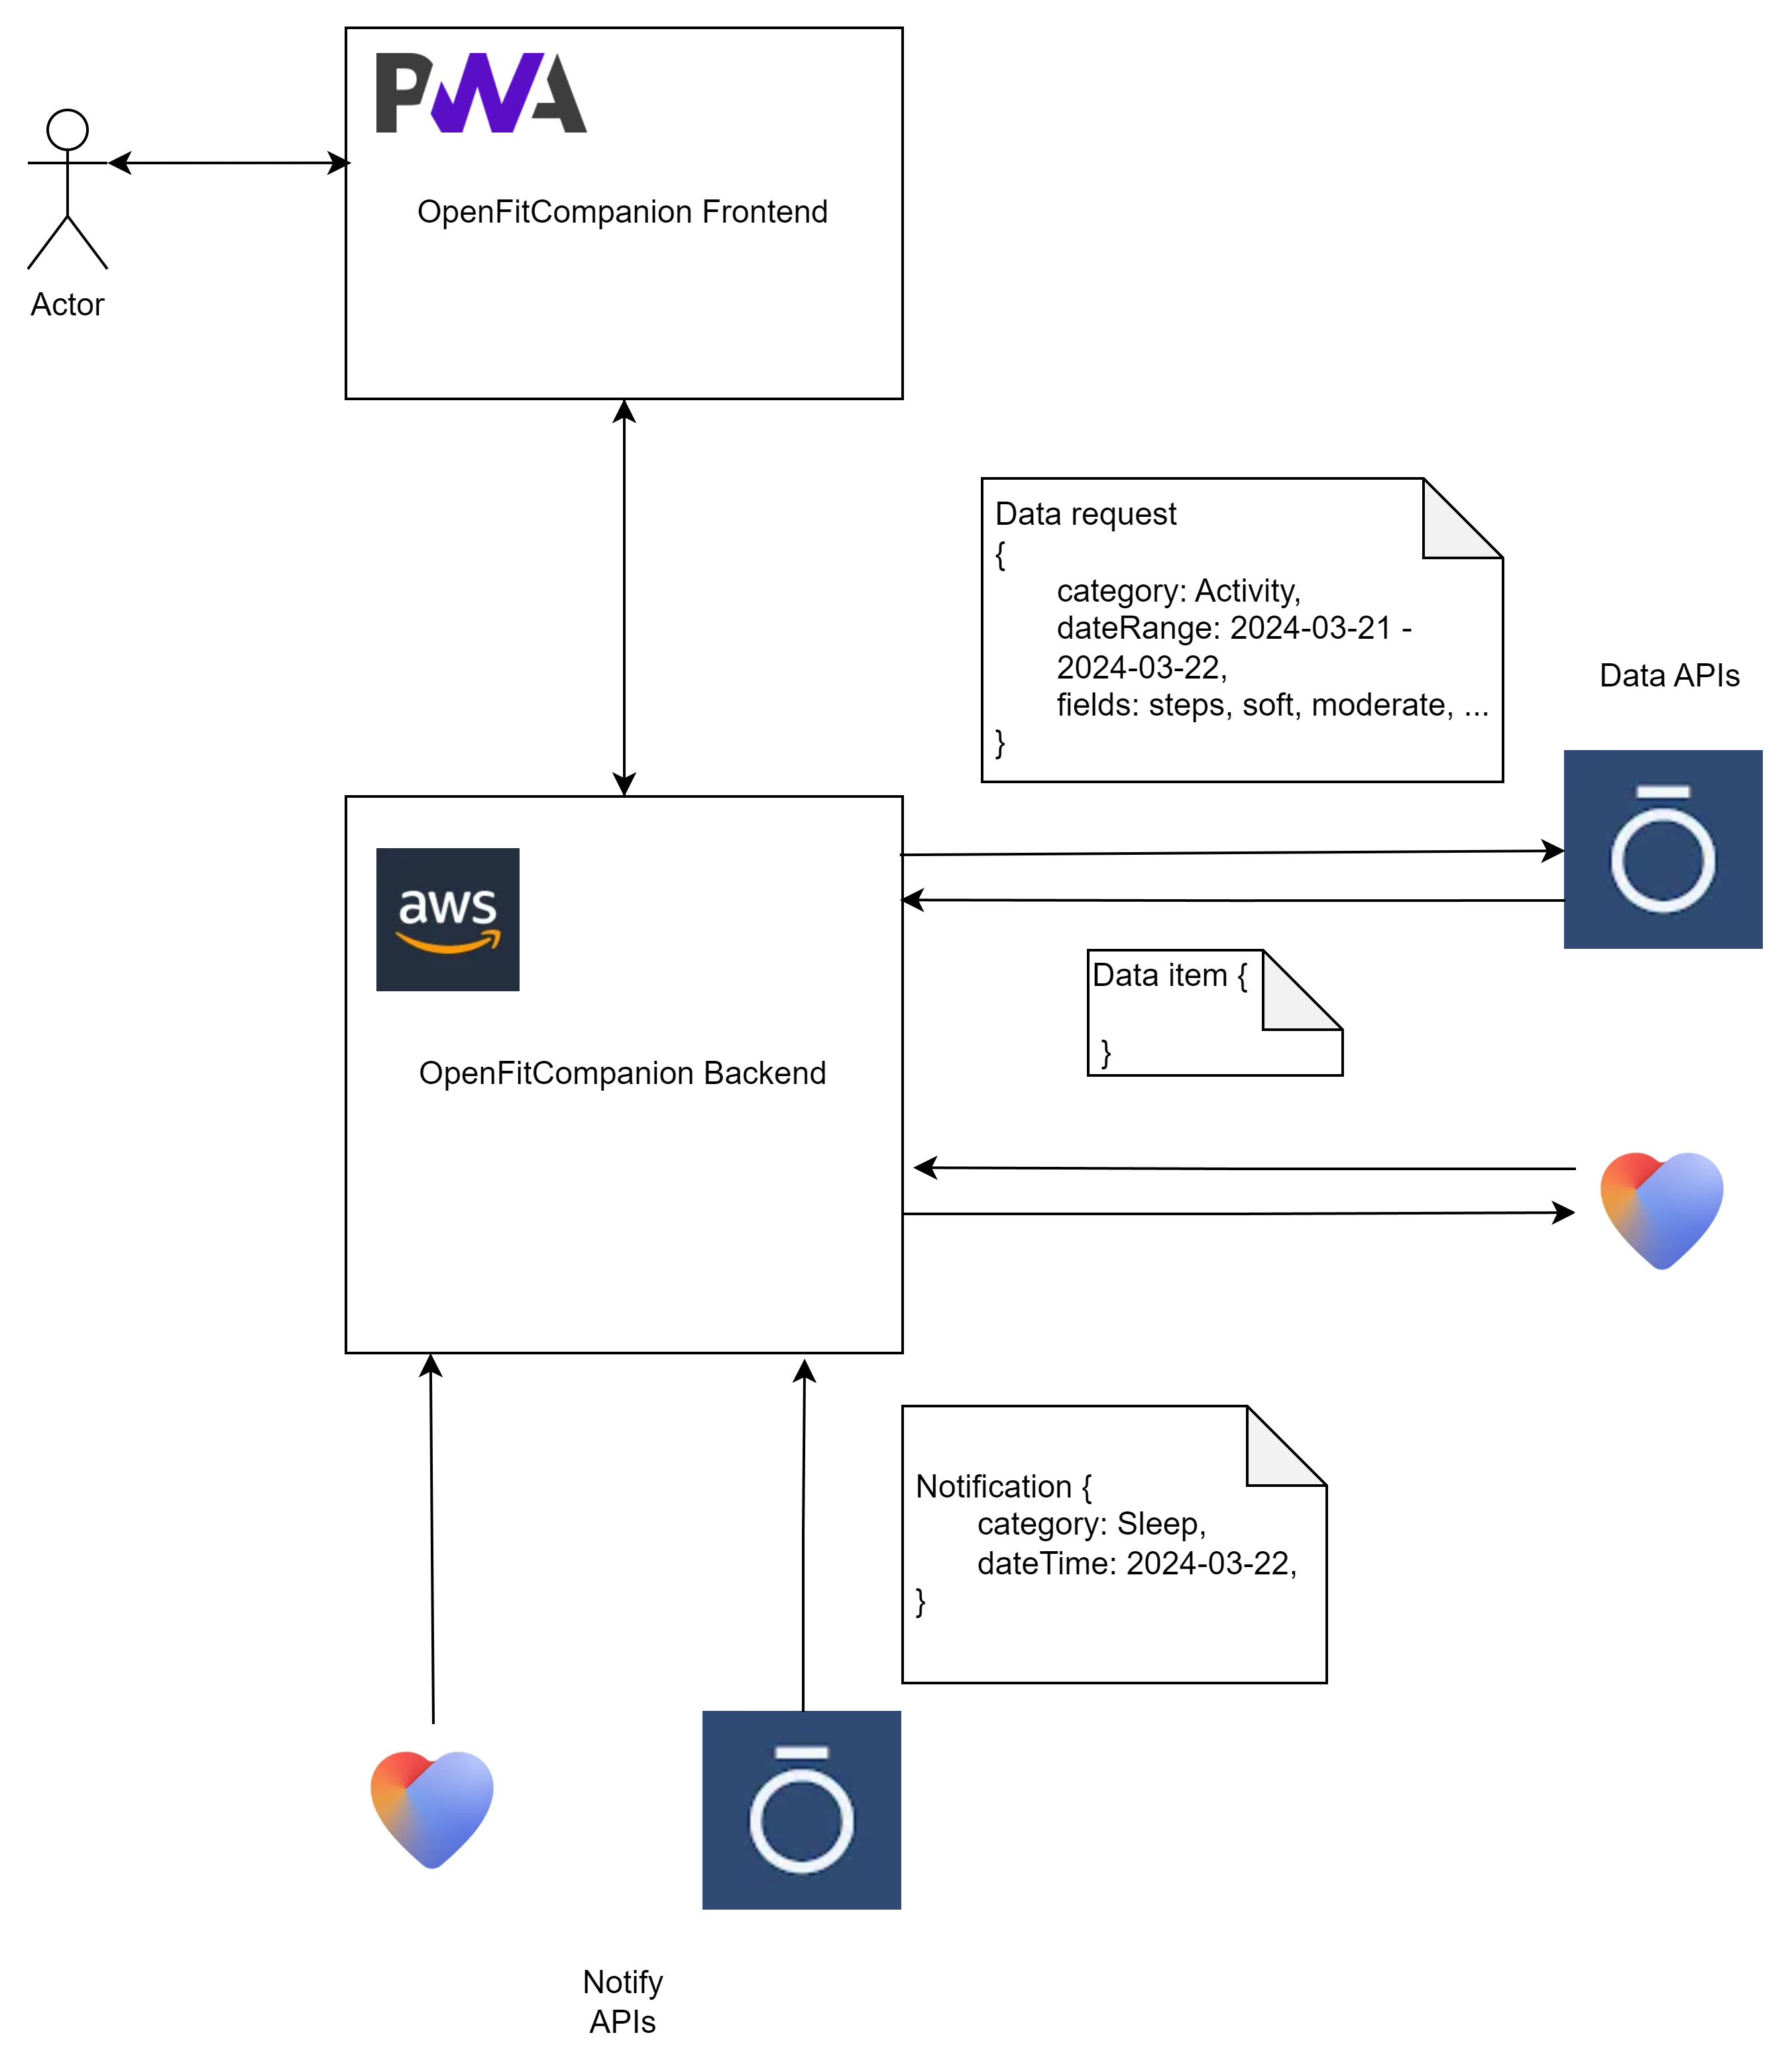
\includegraphics[width=\textwidth,height=\textheight,keepaspectratio]{images/highLevel.png}
    \caption{High-Level architecture diagram}
    \label{fig:1}
\end{figure}
Overall, the architecture is considered event-driven. Computation only needs to happen in response to an external event. This is enabled by providers providing Webhook integrations. Essentially, the backend gets a notification from providers whenever there is new data available from them. The following is the diagram together with sample data exchanged: \ref{fig:1}

Cloud deployed backend service receives notifications from providers, containing information that allows atomic processing of that notification. It does not matter what other requests came before or if any are executing at the moment. 

In response to the notification, backend sends a request to Data APIs of providers, receiving an item(s) back and finally persisting it in a database for further purposes. 

The only requirement for a provider is that they have Data API we can use. Even if a particular provider did not have a webhook (notification) service, we could simply  make data API requests on regular schedule, like every 30 minutes. This would be quite costly if the system was publicly available service, as that scheduled request would be needed for each user. However, for our use case of self-deployed service, the cost would be negligible. However, we still rely on provider's API services to get the actual data from devices. We aren't directly communicating with the smart devices via Bluetooth. So, if a provider does not have such service, we can't integrate their devices into the system. However, all providers examined at least provided Google Fit integration, which could then be used fetch the data indirectly. 

Ultimately, the data is transformed into useful information which is presented to the user through the frontend.

\section{Back-end}
\subsection{AWS services}
\subsection{Adapters}
\subsection{Unifying}
\section{Front-end}
\subsection{UI}
\subsection{Notifying}
\subsection{Reporting}

TODO: Do this chapter
